\documentclass[a4paper]{ltjsarticle}
%preamble.tex

%LaTeXエンジン
\usepackage{luatexja}

%フォント
%\usepackage[ipaex]{luatexja-preset}

%図表
\usepackage{graphicx}
\usepackage{tikz}
\usepackage{multirow}
\usepackage{float}
\usepackage{wrapfig}

%数学
\usepackage{mathtools}
\usepackage{amsmath}

%科学
\usepackage{physics}
\usepackage{siunitx}
\usepackage[version=4]{mhchem}

%リンク
\usepackage{url}

%ハイパーリンク
\usepackage[unicode,hidelinks,pdfusetitle]{hyperref}

%余白
\usepackage[margin=12truemm]{geometry}

%枠付き
\usepackage{ascmac}
\usepackage{fancybox}

%%%%%%%%%%%%%%%%%%%%%%%%%%%%%%%%%%%%%%%%%%%%%%%%%
\begin{document}
\title{北海道大学理学部地球惑星科学科 オープンキャンパス\\クレーター形成実験 解説・問題}
\date{2023年8月6日}
\maketitle
\thispagestyle{empty}

%%%%%%%%%%%%%%%%%%%%%%%%%%%%%%%%%%%%%%%%%%%%%%%%%
\begin{wrapfigure}[23]{r}{70mm}
    \vspace{-8mm}
    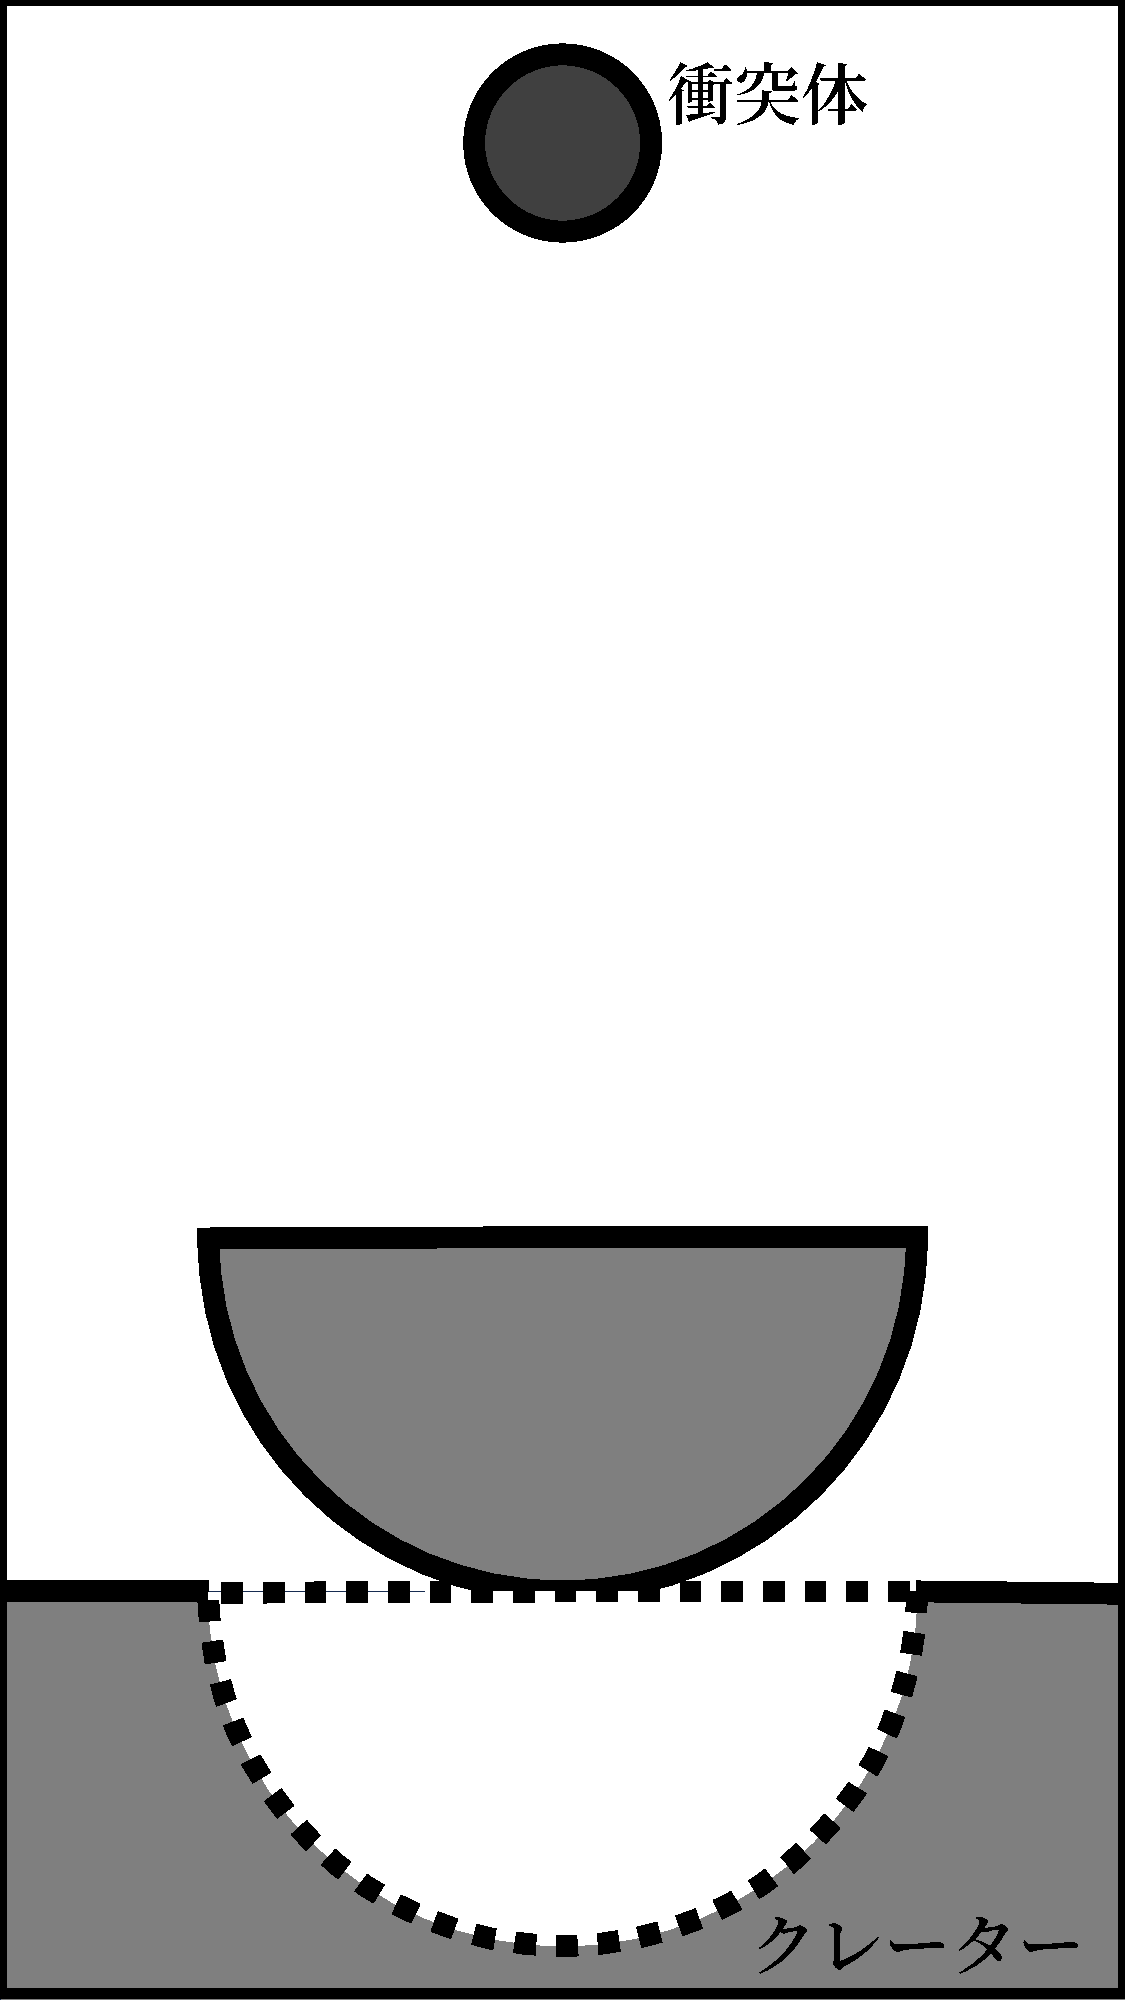
\includegraphics[width=70mm,clip]{./figure/explanation_figure.pdf}
    \vspace{-6mm}
    \caption{クレーター生成過程の模式図}
\end{wrapfigure}
\section{クレーターとは}
クレーター (crater) とは「円形にくぼんだ地形」という意味の言葉です。クレーターは様々な要因で形成され、隕石衝突もその要因の一つです。特に、隕石衝突によってできたクレーターをインパクトクレーターといいます。インパクトクレーターは隕石の衝突エネルギーでつくられます。衝突エネルギーの大きさはクレーターの大きさから推定が可能です。クレーターは太陽系の固体天体の表面に広く見られ、クレーター形成は太陽系の中で普遍的に起こる現象です。そのため、クレーターがどのようにしてできたのかを理解することは,太陽系の固体天体の進化を考える上で重要な要素になります。

\section{問題}
今回のクレーターが半球であると近似してクレーター半径$r$と衝突エネルギー$E$の関係を求めてみましょう。

砂の密度を$\rho$\footnote{$\rho$はギリシャ文字の一つで「ロー」と発音します.}、重力加速度を$g$とします。クレーターをつくるためのエネルギーを、砂地の中の半径$r$の半球を$r$だけそのまま持ち上げるエネルギーで近似します。なぜならば、クレーターができるためには、半球を埋めていた物質がその半球の外に出ていかなければならないからです。そのエネルギーは、半球の質量と$g$と$r$の積で表されます。衝突体の衝突エネルギーがすべてこのエネルギーに変換されたと仮定すると次の等式が成り立ちます。
\begin{equation}
    E = クレーターを作るためのエネルギー.
\end{equation}

以上のことからクレーターの半径$r$と衝突エネルギー$E$の関係式を求めてください。
\vspace{-0.8em}
\begin{itemize}
    \item[※] 実際のクレーター形成では地殻の破砕や加熱にもエネルギーが使われます。また大きなクレーターでは斜面の崩壊等によりクレーターの変形が起きます。そのため、この結果を月のクレーターなどに外挿するには注意が必要です。
    \item[※]裏面に回答してください。
    \item[※]不明な点があれば遠慮なく担当者に質問してください。
\end{itemize}

\section*{参考文献}
\begin{itemize}
    \item 松井孝典ほか. 2011. 比較惑星学. 地球惑星科学 12. 東京: 岩波書店.
    \item 佐々木晶ほか. 2019. 太陽・惑星系と地球. 現代地球科学入門シリーズ 1. 東京: 共立出版.
\end{itemize}

\end{document}